\documentclass[12pt,a4paper]{article}
\usepackage{../lecture-notes/vkCourseML}
\usepackage{lipsum}
\usepackage{indentfirst}
\title{Машинное обучение, ФКН ВШЭ\\Семинар №6}
\author{}
\date{}
\begin{document}
	\maketitle
\section{Предсказание вероятностей}
\par Разберемся, каким требованиям должен удовлетворять классификатор, чтобы его выход можно было расценивать как оценку вероятности класса.

\par Пусть в каждой точке~$x \in \mathbb{X}$ пространства объектов
задана вероятность~$p(y=+1 \cond x)$ того, что данный объект относится
к классу $+1$, и пусть алгоритм~$b(x)$ возвращает числа из отрезка~$[0, 1]$. Потребуем, чтобы эти предсказания пытались в каждой точке~$x$ приблизить вероятность положительного класса~$p(y = +1 | x)$.
\par Разумеется, выполнение этого требования зависит от функции потерь~---
минимум ее матожидания в каждой точке~$x$ должен достигаться на данной вероятности:
$$\arg \min_{b \in \mathbb{R}} \mathbb{E} \left[ L(y, b)|x \right] = p(y=+1|x).$$

\begin{vkProblem}
	Покажите, что квадратичная функция потерь~$L(y, b) = ([y = +1] - b)^2$
	позволяет предсказывать корректные вероятности.
\end{vkProblem}


\begin{esSolution}
	Заметим, что поскольку алгоритм возвращает числа от 0 до 1,
	то его ответ должен быть близок к единице, если объект относится
	к положительному классу, и к нулю~--- если объект относится
	к отрицательному классу.
	
	Запишем матожидание функции потерь в точке~$x$:
	$$\mathbb{E} \left[ L(y, b)|x\right] = p(y=+1|x)(b-1)^2 + (1 - p(y=+1|x))(b-0)^2.$$
	Продифференцируем по~$b$:
	$$\frac{\partial}{\partial b}
	\mathbb{E} \left[
	L(y, b)
	|
	x
	\right] =
	2 p(y = +1 | x) (b - 1)
	+
	2 (1 - p(y = +1 | x)) b
	=
	2b - 2p(y = +1 | x)
	=
	0.$$
	Легко видеть, что оптимальный ответ алгоритма действительно
	равен вероятности:
	$$b = p(y = +1 | x).$$
\end{esSolution}

\begin{vkProblem} Покажите, что абсолютная функция потерь~$L(y, b) = |[y = +1] - b|, \, b \in [0; 1],$
	не позволяет предсказывать корректные вероятности.
\end{vkProblem}
\begin{esSolution}
	Запишем матожидание функции потерь в точке~$x$:
	\begin{align*}
		\mathbb{E} \left[ L(y, b)|x\right] = &p(y=+1|x)|1-b| + (1 - p(y=+1|x))|b| = \\
		&= p(y=+1|x)(1-b)+ (1 - p(y=+1|x))b.\\
	\end{align*}
	Продифференцируем по~$b$:
	$$\frac{\partial}{\partial b}
	\mathbb{E} \left[
	L(y, b)
	|
	x
	\right] =
	1 - 2 p(y = +1 | x) = 0.$$
	Рассмотрим 2 случая:
	\begin{enumerate}
		\item $p(y=+1|x) = \frac{1}{2}.$ Тогда $\mathbb{E} \left[ L(y, b)|x\right] = \frac{1}{2} \quad \forall b \in [0; 1],$ а потому классификатор не позволяет предсказывать корректную вероятность в точке $x$.
		\item $p(y=+1|x) \ne \frac{1}{2}.$ В этом случае интервал $(0; 1)$ не содержит критических точек, а потому минимум матожидания достигается на одном из концов отрезка $[0; 1]:$
		\begin{align*}
			\min_{b \in [0;1]} \mathbb{E} \left[ L(y, b)|x\right] = 
			\min \left(\mathbb{E} \left[ L(y, 0)|x\right], \mathbb{E} \left[ L(y, 1)|x\right] \right) =\\
			\min \left(p(y = +1 | x), 1 - p(y = +1 | x)\right).
		\end{align*}
		Отсюда $\arg \min_{b \in [0;1]} \mathbb{E} \left[ L(y, b)|x\right] \in \{0, 1\},$ а потому классификатор также не позволяет предсказывать корректную вероятность в точке $x$.
	\end{enumerate}
\end{esSolution}

\section{Калибровка вероятностей}

Часто при обучении моделей для бинарной классификации хочется получать не только предсказанную метку класса, но и вероятность положительного класса. Предсказанная вероятность может служить как мера уверенности нашего алгоритма. Однако некоторые алгоритмы не выдают корректные вероятности классов. В таком случае калибруют вероятности модели.

Для начала определимся с тем, что хотим получить от предсказанных вероятностей. В задаче бинарной классификации откалиброванным алгоритмом называют такой алгоритм, для которого доля положительных примеров (на основе реальных меток классов) для предсказаний в окрестности произвольной вероятности $p$ совпадает с этим значением $p$. Например, если взять объекты, для которых предсказанные вероятности близки к 0.7, то окажется, что среди них 70\% принадлежат положительному классу. Нет критерия, которое бы установило откалиброванность алгоритма, однако можно построить калибровочную кривую. На этой кривой абсцисса точки соответствуют значению $p$ (предсказаний алгоритма), а ордината соответствует доле положительных примеров, для которых алгоритм предсказал вероятность, близкую к $p$. В идеальном случае эта кривая совпадает с прямой $y = x$. Примеры такой кривой на рис. (\ref{fig:plot}).

\begin{center}
\begin{figure}[!htb]
 \centering
 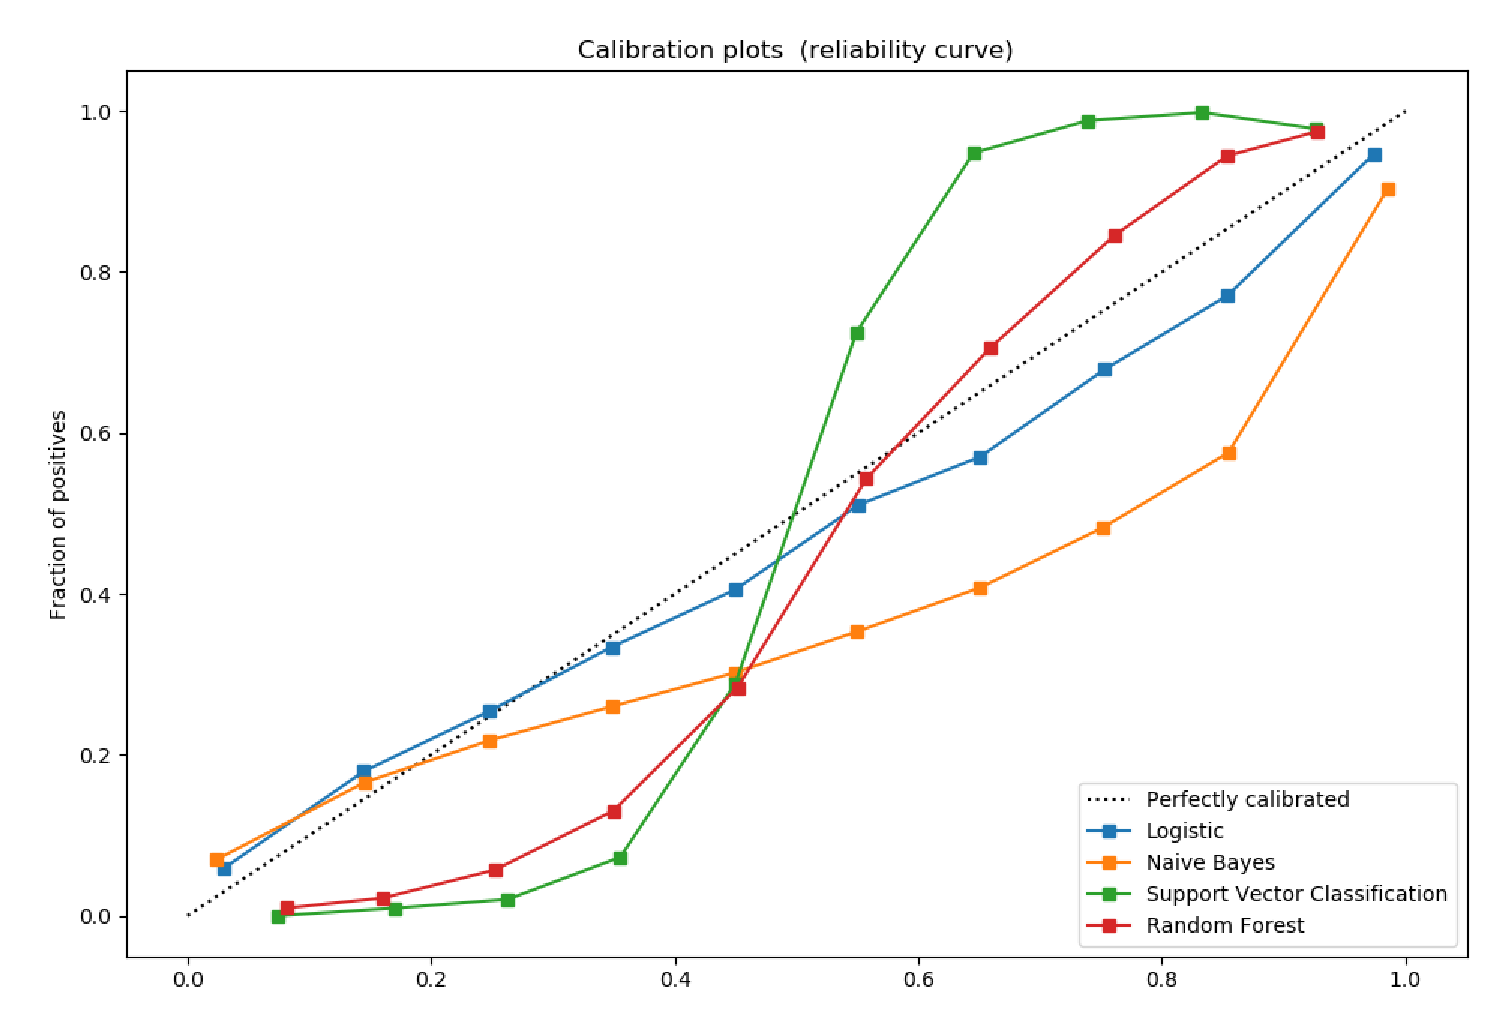
\includegraphics[width=0.7\linewidth]{img/calibration_plot.eps}
 \caption{Калибровочные кривые нескольких алгоритмов}\label{fig:plot}
\end{figure}
\end{center}

Изучим два стандартных метода для калибровки вероятностей алгоритма: калибровка Платта и изотоническая регрессия.

\subsection{Калибровка Платта}

Пусть наш алгоритм выдаёт значения $f(x)$ (могут не быть вероятностями). Тогда итоговая вероятность:

$$P(y = 1 | x) = \frac{1}{1+\exp (af(x) + b)},$$

где $a, b$ -- скалярные параметры. Эти параметры настраиваются методом максимума правдоподобия (минимизируя логистическую функцию потерь) на отложенной выборке или с помощью кросс валидации. Также Платт предложил настраивать параметры на обучающей выборке базовой модели, а для избежания переобучения изменить метки объектов на следующие значения:

$$t_{+} = \frac{N_{+} + 1}{N_{-} + 2}$$ для положительных примеров и

$$t_{-} = \frac{1}{N_{-} + 2}$$ для отрицательных.

Калибровку Платта можно представить как применения логистической регрессии поверх предсказаний другого алгоритма с отключенной регуляризацией.


\subsection{Изотоническая регрессия}

В этом методе также строится отображение из предсказаний модели в откалиброванные вероятности. Для этого используем изотоническую функцию (неубывающая кусочно-постоянная функция), в которой $x$ -- выходы нашего алгоритма, а $y$ -- целевая переменная. Иллюстрация изотонической регрессии на рис. (\ref{fig:isotonic}).

Мы хотим найти такую функцию $m(t)$: $P(y = 1 | x) = m(f(x))$. Она настраивается под квадратичную ошибку:

$$m = \argmin_{z} \sum (y_i - z(f(x_i))^2,$$

с помощью специального алгоритма (Pool-Adjacent-Violators Algorithm), изучать который в этом курса не будем.

\begin{center}
\begin{figure}[!htb]
 \centering
 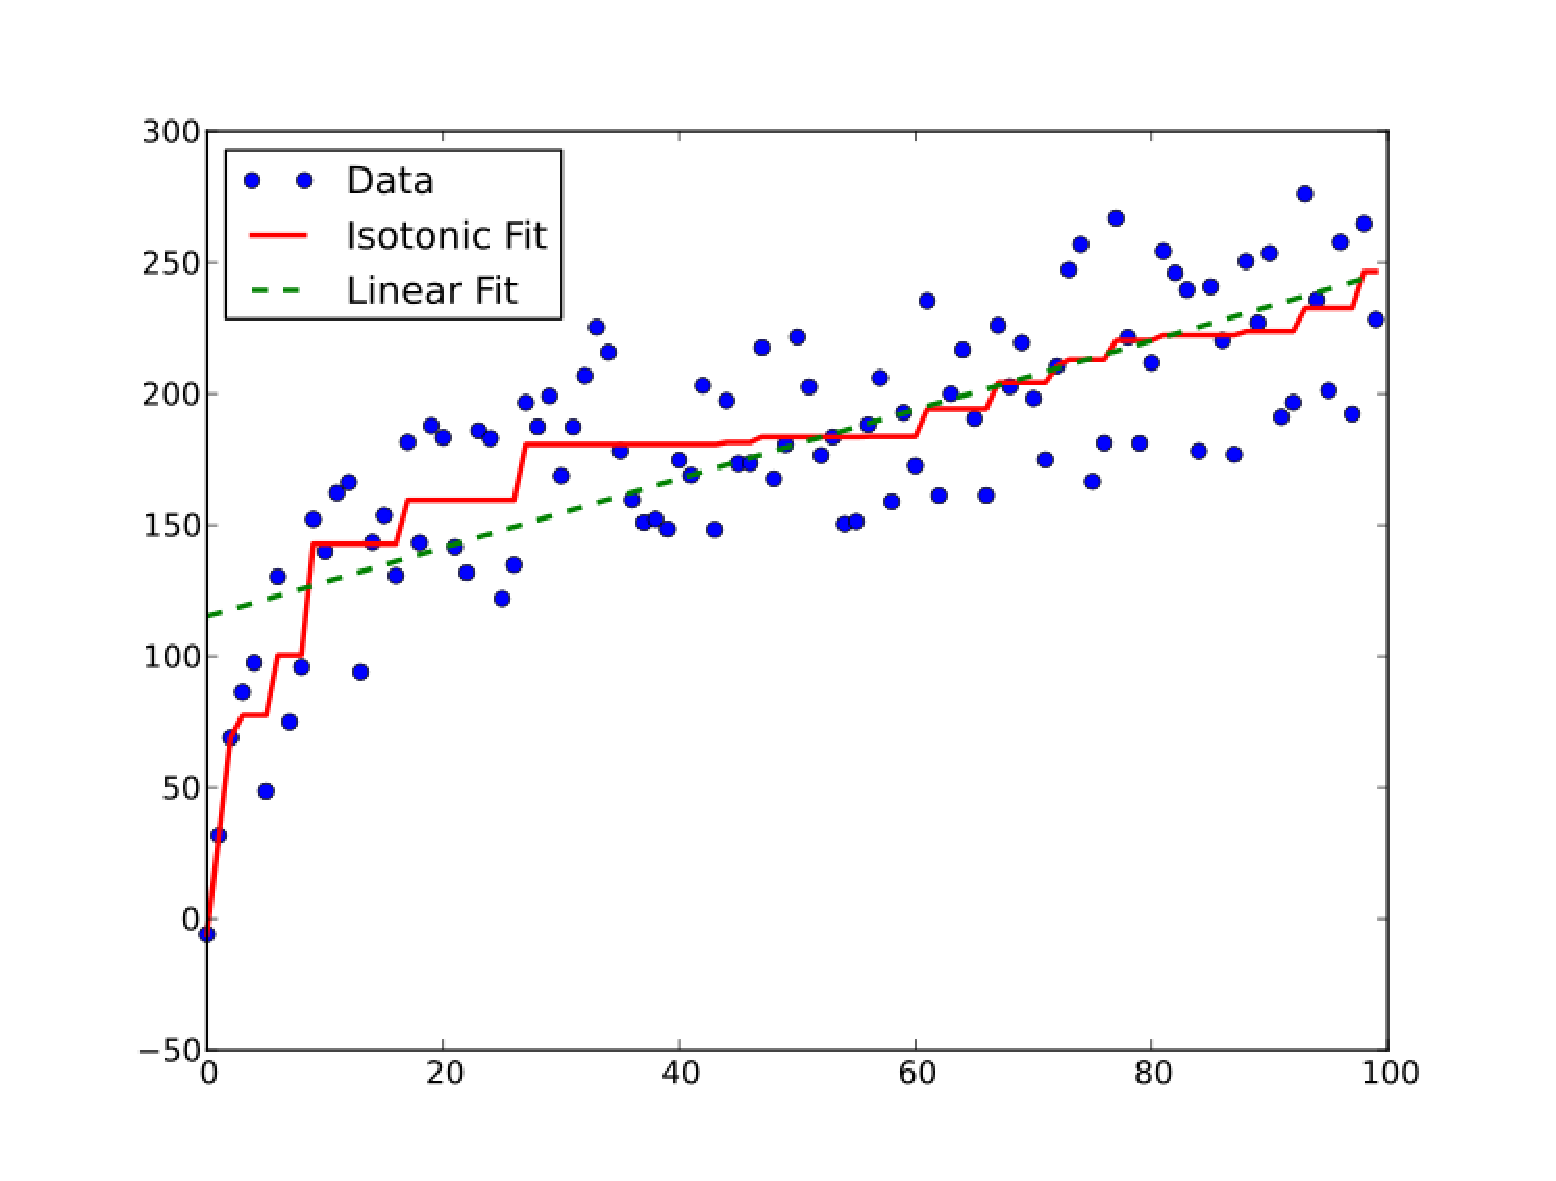
\includegraphics[width=0.7\linewidth]{img/isotonic.eps}
 \caption{Изотоническая регрессия}\label{fig:isotonic}
\end{figure}
\end{center}


В результате калибровки получаем надстройку над нашей моделью, которая применяется поверх предсказаний базовой модели. В случае мультиклассовой классификации каждый класс калибруется отдельно против остальных (one-versus-all), вероятности при предсказании нормируются.


\section{Квантильная регрессия}

В некоторых задачах цены занижения и завышения прогнозов могут отличаться друг от друга.
Например, при прогнозировании спроса на товары интернет-магазина гораздо опаснее заниженные
предсказания, поскольку они могут привести к потере клиентов.
Завышенные же прогнозы приводят лишь к издержкам на хранение товара на складе.
Функционал в этом случае можно записать как
\[
    Q(a, X^\ell)
    =
    \sum_{i = 1}^{\ell}
        \rho_\tau(y_i - a(x_i)),
\]
где
\[
    \rho_\tau(z)
    =
    (\tau - 1) [z < 0] z
    +
    \tau [z \geq 0] z
    =
    (\tau - \frac{1}{2})z + \frac{1}{2} |z|,
\]
а параметр~$\tau$ лежит на отрезке~$[0, 1]$ и определяет
соотношение важности занижения и завышения прогноза.
Чем больше здесь~$\tau$, тем выше штраф за занижение прогноза.

Обсудим вероятностный смысл данного функционала.
Будем считать, что в каждой точке~$x \in \XX$ пространства объектов
задано вероятностное распределение~$p(y \cond x)$ на возможных ответах для данного объекта.
Такое распределение может возникать, например, в задаче предсказания кликов по рекламным баннерам:
один и тот же пользователь может много раз заходить на один и тот же сайт и видеть данный баннер;
при этом некоторые посещения закончатся кликом, а некоторые~--- нет.

Известно, что при оптимизации квадратичного функционала алгоритм~$a(x)$
будет приближать условное матожидание ответа в каждой точке пространства
объектов:~$a(x) \approx \EE [y \cond x]$;
если же оптимизировать среднее абсолютное отклонение, то итоговый алгоритм
будет приближать медиану распределения:~$a(x) \approx \text{median} [p(y \cond x)]$.
Рассмотрим теперь некоторый объект~$x$ и условное распределение~$p(y \cond x)$.
Найдем  число~$q$, которое будет оптимальным с точки зрения нашего функционала:
\[
    Q = \int_\YY \rho_\tau(y - q) p(y \cond x) dy.
\]
Продифференцируем его~(при этом необходимо воспользоваться правилами
дифференцирования интегралов, зависящих от параметра):
\[
    \frac{\partial Q}{\partial q}
    =
    (1 - \tau) \int_{-\infty}^{q} p(y \cond x) dy
    -
    \tau \int_{q}^{\infty} p(y \cond x) dy
    =
    0.
\]
Получаем, что
\[
    \frac{\tau}{1 - \tau}
    =
    \frac{
        \int_{-\infty}^{q} p(y \cond x) dy
    }{
        \int_{q}^{\infty} p(y \cond x) dy
    }.
\]
Данное уравнение будет верно, если~$q$ будет равно~$\tau$-квантили распределения~$p(y \cond x)$.
Таким образом, использование функции потерь~$\rho_\tau(z)$ приводит к тому,
что алгоритм~$a(x)$ будет приближать~$\tau$-квантиль распределения ответов в каждой точке
пространства объектов.

\end{document}
